\documentclass[10pt,twocolumn]{article}

% ---------- Page geometry (IEEE-conference-like) ----------
\usepackage[letterpaper,top=0.75in,bottom=1in,left=0.625in,right=0.625in,columnsep=0.25in]{geometry}
\usepackage{times}
\usepackage[T1]{fontenc}
\usepackage[utf8]{inputenc}
\usepackage{graphicx}
\usepackage{tikz}
\usetikzlibrary{arrows.meta,positioning,shapes.geometric,shapes.symbols,fit,backgrounds,calc}
\usepackage{booktabs}
\usepackage{array}
\usepackage{caption}
\usepackage{amsmath}
\usepackage{balance}
\usepackage{enumitem}
\usepackage{fancyvrb}
\fvset{fontsize=\small}
\setlist[itemize]{leftmargin=*,itemsep=0pt,topsep=1pt,parsep=0pt}
\usepackage{titlesec}
\usepackage{xcolor}

\captionsetup{font=small,labelfont=bf,skip=4pt}
\renewcommand{\arraystretch}{1.15}

% ---------- Section formatting ----------
\titleformat{\section}{\centering\normalsize\bfseries}{\Roman{section}.}{0.6em}{\MakeUppercase}
\titlespacing*{\section}{0pt}{10pt}{6pt}
\titleformat{\subsection}{\normalsize\itshape}{\Alph{subsection}.}{0.5em}{}
\titlespacing*{\subsection}{0pt}{6pt}{2pt}
\titleformat{\subsubsection}{\normalsize\bfseries}{}{0em}{}
\titlespacing*{\subsubsection}{0pt}{5pt}{2pt}

\setlength{\abovecaptionskip}{4pt}
\setlength{\belowcaptionskip}{2pt}
\setlength{\textfloatsep}{8pt plus 2pt minus 2pt}
\setlength{\intextsep}{6pt plus 2pt minus 2pt}
\setlength{\floatsep}{6pt plus 2pt minus 2pt}
\raggedbottom

\pagestyle{plain}
\setlength{\parindent}{1em}
\setlength{\parskip}{0pt}

\newcommand{\ieeeabstract}[1]{\noindent{\bfseries \emph{Abstract}---}#1}
\newcommand{\ieeeindex}[1]{\noindent{\bfseries \emph{Index Terms}---}#1}

% ---------- Colors for module/workflow diagrams ----------
\definecolor{navyblue}{RGB}{22,54,92}
\definecolor{stepblue}{RGB}{58,112,166}
\definecolor{stepteal}{RGB}{60,150,150}
\definecolor{steporange}{RGB}{224,140,60}
\definecolor{stepgreen}{RGB}{70,150,90}
\definecolor{wireframegray}{RGB}{120,120,120}

\begin{document}

% ================= TITLE =================
\twocolumn[
\begin{center}
{\LARGE\bfseries Smart Real Estate Rental Platform: A Full-Stack Web Architecture for Property Discovery and Broker--User Connectivity}\\
\vspace{10pt}
{\large Hemik Patel, Krushil Tejani, Namra Tejani, Dhruvsinh Barad}\\
\vspace{4pt}
{\itshape Department of Computer Science and Engineering}\\
{\itshape Parul Institute of Engineering and Technology, Parul University, Vadodara, Gujarat, India}\\
\vspace{2pt}
{\itshape Guide: Prof. Kapil Agrawal}\\
\vspace{10pt}
\end{center}
\begin{minipage}{\textwidth}
\small
\ieeeabstract{Renting or buying a property in a typical Indian city still involves comparing listings across several unrelated portals and confirming availability over the phone, because no single source is treated as authoritative. This paper presents the Smart Real Estate Rental Platform, a full-stack MERN (MongoDB, Express.js, React.js, Node.js) application that centralizes property listings, structured broker profiles, and enquiry handling behind a single role-aware interface. We reviewed recent MERN-based rental and real-estate platforms reported in the literature and identified four recurring gaps: search and enquiry are rarely linked as a persistent, queryable record; the indexing strategy behind filtered search is rarely specified or justified against real query patterns; role-based authorization is described but rarely verified at the server boundary rather than only hidden in the UI; and administrative oversight across an entire platform, rather than a single owner's listings, is rarely treated as a first-class module. The Smart Real Estate Rental Platform addresses these four gaps through a \texttt{Lead} collection that persistently links tenant, broker, and property; a compound- and geospatial-indexed \texttt{Properties} schema matched to the platform's actual filter combinations; JWT-based authentication with server-side role middleware enforced on every protected route; and a dedicated administrator module with cross-broker visibility. The system was evaluated through structured functional testing across authentication, listing management, filtered search, favorites, and the enquiry pipeline; every tested workflow produced the expected result on a development-scale dataset, though the platform has not yet been evaluated under concurrent load or at production scale. We discuss the resulting limitations honestly and outline machine-learning-based recommendation, real-time chat, and formal load testing as realistic next steps rather than implemented features.}
\vspace{4pt}

\ieeeindex{Real Estate Platform, MERN Stack, MongoDB Indexing, Broker--User Connectivity, Role-Based Access Control, Property Discovery, REST API, JWT Authentication}
\vspace{8pt}
\end{minipage}
]

% ================= I. INTRODUCTION =================
\section{Introduction}

Online property search in India has grown considerably, yet renting a place still involves a surprising amount of manual cross-checking. A tenant looking for a two-bedroom flat under a fixed budget typically opens two or three listing portals, applies roughly the same filters on each, and still calls brokers directly because a listing shown as available on one site is already gone by the time it is followed up on. Property owners and brokers face a mirror version of the same problem: without a structured way to manage listings and enquiries, tracking which unit has been shown to which prospective tenant becomes a manual bookkeeping exercise carried out over phone calls and forwarded messages.

Two developments make a more structured approach practical today. First, document-oriented databases such as MongoDB let a single schema describe rental flats, sale plots, and short-stay listings without forcing every property into the same rigid set of columns. Second, mature open-source tooling around the MERN stack -- React for the interface, Express and Node.js for the API layer, JWT for stateless authentication -- makes it realistic for a small team to build a role-aware, database-backed platform without a large services budget.

This paper presents the Smart Real Estate Rental Platform, a system built to close two structural gaps directly: the absence of a single, filterable, consistently-updated source of property information, and the absence of a persistent link between a tenant's enquiry, the broker who owns the listing, and the property itself.

% ================= II. LITERATURE REVIEW =================
\section{Literature Review}

\textit{Review Methodology:} A search across IEEE Xplore, ScienceDirect, SpringerLink, and Google Scholar was performed with emphasis on 2022--2026, using the terms: MERN stack real estate platform, MongoDB indexing strategy, JWT REST API security, PropTech digital transformation, and rental property management system. Eight sources most directly relevant to the platform's architecture and data layer were retained for detailed comparison; broader PropTech and digital-transformation literature was used to frame the problem statement in Section~III.

\textit{MERN-Stack Rental and Real-Estate Platforms:} Several recent student and early-career projects describe MERN-based rental or real-estate applications. Kalbande et al.~\cite{kalbande2023} describe a smart house rental management system built on similar principles. Khan et al.~\cite{khan2025} present RENTEASE, a MERN rental platform that additionally proposes lease-agreement management and rent-payment tracking, alongside an aspirational reference to AI-driven tenant matching that is described as a future direction rather than a validated component. Kumar et al.~\cite{kumar2024} describe a house rental application with JWT authentication, a searchable property database, and a wishlist feature comparable in scope to the favorites mechanism described in Section~V-E. None of these three systems describes an indexing strategy for the underlying document store, and none reports how role separation between owners and tenants is enforced at the server rather than only in the interface.

\textit{Database and Indexing Approaches:} Work specifically on MongoDB query optimization~\cite{nuriev2024,tao2024} establishes that compound-index field ordering materially affects whether a filtered query can use an index at all, and that indexing decisions should be driven by actual query shape rather than applied uniformly across every field. This principle informs the indexing strategy in Section~V-C but is rarely referenced in the application-level rental-platform literature reviewed above.

\textit{Authentication and Authorization:} JWT-based stateless authentication for REST APIs is well studied~\cite{neumann2021,dalimunthe2023}, and the general pattern -- sign a token at login, verify it on every protected request -- is consistent across the rental-platform papers reviewed. However, these papers describe role differentiation (tenant vs.\ owner vs.\ administrator) at the level of what each role can \emph{see} in the interface, without describing whether the corresponding API routes independently reject a request from the wrong role.

\subsection{Research Gaps}
Based on the above review, four recurring gaps were identified in the MERN-based rental-platform literature:

\smallskip
\noindent\textbf{Gap 1 --- Search and Enquiry Are Rarely Linked as a Persistent Record.} Reviewed platforms implement property search and an enquiry or contact form as separate features. None of them persist a structured record connecting a specific tenant, a specific broker, and a specific property over time, which means neither side can later answer ``who already asked about this listing'' without searching through messages or call logs.

\smallskip
\noindent\textbf{Gap 2 --- Indexing Strategy Is Rarely Specified or Justified.} Filtering and search are described functionally (``users can filter by price and location'') but the underlying compound-index design that keeps such filtering responsive as the listing count grows is not discussed in any of the three MERN rental-platform papers reviewed, despite established guidance that field order in a compound index determines whether it is usable for a given query~\cite{nuriev2024}.

\smallskip
\noindent\textbf{Gap 3 --- Role-Based Authorization Is Described but Not Verified at the Server Boundary.} Role separation is presented as a UI concern (hiding an ``Edit'' button from non-owners) more often than as a server-enforced constraint. None of the reviewed papers reports explicit testing of what happens when a request from the wrong role reaches a protected route directly, bypassing the UI.

\smallskip
\noindent\textbf{Gap 4 --- Administrative Oversight Across an Entire Platform Is Rarely a First-Class Module.} Reviewed systems focus on the tenant-facing search experience or a single owner's listing dashboard. None describes a dedicated administrator view that aggregates users, listings, and enquiries \emph{across} brokers, which is what would be needed to answer platform-level operational questions rather than a single user's questions.

\begin{table}[t]
\centering
\caption{Summary of Research Gaps}
\label{tab:gaps}
\small
\begin{tabular}{@{}p{3.7cm}p{3.7cm}@{}}
\toprule
\textbf{Missing in Literature} & \textbf{This Platform's Response} \\
\midrule
Search and enquiry treated as separate, unlinked features & \texttt{Lead} document persistently links tenant, broker, and property \\
Indexing strategy rarely specified or justified against query patterns & Compound indexes chosen to match the platform's actual filter combinations (Sec.~V-C) \\
Role separation enforced only in the UI, not verified server-side & JWT role middleware runs on every protected route; tested directly against wrong-role requests \\
No cross-broker administrative oversight module & Dedicated admin module aggregating users, listings, and leads platform-wide \\
\bottomrule
\end{tabular}
\end{table}

% ================= III. PROBLEM STATEMENT =================
\section{Problem Statement}

Fragmented listing data carries a real cost even though it is not the kind of cost that shows up in a single measurable incident. Systematic reviews of digital transformation in real estate report that operational and interaction-focused tools (virtual tours, cloud communication, digital documentation) have been adopted unevenly across agencies, while more integrated PropTech platforms have seen slower adoption due to cost and organizational constraints~\cite{digitaltransform2025}, leaving a large share of day-to-day rental activity dependent on manual coordination between individual brokers and tenants. Separately, sector analyses describe a persistent gap between how important digital tools are considered and how deeply they are actually integrated into daily property-management operations~\cite{proptechmismatch2026}.

For a tenant, this translates into repeating the same search across multiple portals and confirming availability by phone because no listing source is treated as reliably current. For a broker or owner, it means enquiries arrive through disconnected channels (phone calls, messaging apps, contact forms on different sites) with no shared record of which prospective tenant has already been contacted about which property. For a platform operator, it means there is no single place to answer operational questions -- how many active listings exist, how many enquiries are open, which brokers are responsive -- without manually cross-referencing several data sources.

The problem this platform addresses is therefore threefold: (1) the absence of a single, structured, filterable source of property data that supports the query patterns tenants actually use; (2) the absence of a persistent, queryable link between a tenant's enquiry, the responsible broker, and the property in question; and (3) the absence of a consolidated administrative view of platform activity that does not require direct database inspection.

% ================= IV. PROPOSED METHODOLOGY =================
\section{Proposed Methodology}

\textit{System Overview:} The platform is a closed request-response pipeline: a tenant, owner/broker, or administrator interacts with a React interface, which issues a REST request to an Express API; the request passes through authentication and role-check middleware before reaching a controller, which executes a Mongoose query or write against MongoDB and returns a JSON response. The same pipeline handles every resource (properties, leads, favorites, users), differing only in which controller and which role check apply.

\textit{Property Ingestion and Validation:} When an owner or broker submits a listing, the backend validates required fields (title, price, property type, listing type, city, address, contact number) using Mongoose schema-level constraints before the document is written with an initial \texttt{status} of \texttt{active}. Optional fields that apply only to certain property types (\texttt{dailyPrice} for short-stay listings, \texttt{indoorOutdoor} and \texttt{parkingAvailable} for applicable property types) are simply omitted from documents where they do not apply.

\textit{Search Query Construction:} A search request arrives as a set of optional filter parameters. The controller builds a MongoDB filter object incrementally, adding a condition only for parameters actually supplied, and always constraining \texttt{status} to \texttt{active} so inactive listings never surface in tenant-facing results. This filter is executed against the compound indexes described in Section~V-C.

\textit{Listing Relevance Score:} When a tenant does not specify an explicit sort order, listings are ordered by a weighted relevance score rather than by raw insertion order, so that recently added and platform-featured listings surface ahead of older, unfeatured ones:
\begin{equation}
R = w_f \cdot F + w_r \cdot \hat{r} + w_v \cdot \hat{v}
\label{eq:relevance}
\end{equation}
where $F \in \{0,1\}$ indicates whether a listing is marked \texttt{isFeatured}, $\hat{r} \in [0,1]$ is the listing's recency, min--max normalized against the current search result set, $\hat{v} \in [0,1]$ is its normalized view count, and $w_f, w_r, w_v$ are configurable weights (used here as $w_f=0.5$, $w_r=0.3$, $w_v=0.2$) that can be tuned without changing the underlying query shape.

\textit{Lead Aging for Administrative Review:} To surface enquiries that a broker has not yet acted on, each open lead's age is computed as
\begin{equation}
A(\ell) = t_{\text{now}} - t_{\text{created}}(\ell)
\label{eq:aging}
\end{equation}
and a lead is flagged for administrative attention when $A(\ell) > \tau$ for a configurable threshold $\tau$ (for example, 48 hours), rather than requiring an administrator to manually scan every broker's lead list to find enquiries that have gone unanswered.

% ================= V. SYSTEM ARCHITECTURE =================
\section{System Architecture}

The platform consists of six interconnected modules: authentication and authorization, property management, search and discovery, the enquiry (lead) pipeline, favorites, and administrative oversight. Fig.~\ref{fig:pipeline} shows how a request moves through these modules regardless of which resource it targets.

\begin{figure}[t]
\centering
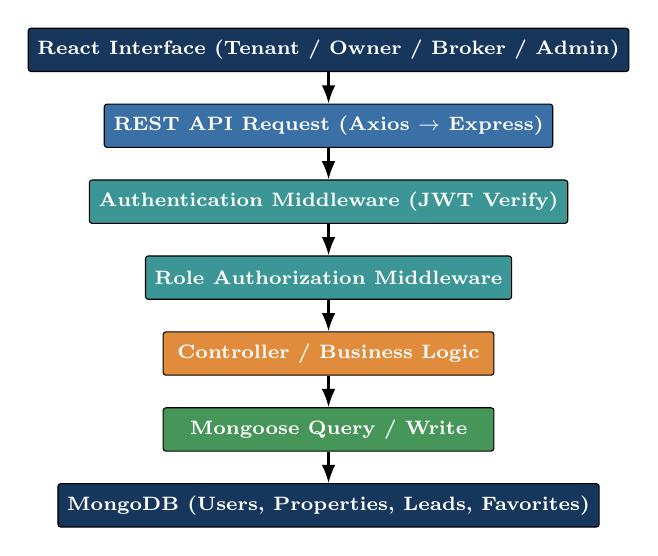
\begin{tikzpicture}[
  node distance=4mm,
  box/.style={draw, rounded corners=1pt, minimum width=4.2cm, minimum height=0.55cm, align=center, font=\scriptsize\bfseries, text=white, fill=stepblue},
  >=Latex
]
\node[box, fill=navyblue] (n1) {React Interface (Tenant / Owner / Broker / Admin)};
\node[box, below=of n1] (n2) {REST API Request (Axios $\rightarrow$ Express)};
\node[box, below=of n2, fill=stepteal] (n3) {Authentication Middleware (JWT Verify)};
\node[box, below=of n3, fill=stepteal] (n4) {Role Authorization Middleware};
\node[box, below=of n4, fill=steporange] (n5) {Controller / Business Logic};
\node[box, below=of n5, fill=stepgreen] (n6) {Mongoose Query / Write};
\node[box, below=of n6, fill=navyblue] (n7) {MongoDB (Users, Properties, Leads, Favorites)};
\foreach \a/\b in {n1/n2,n2/n3,n3/n4,n4/n5,n5/n6,n6/n7}
  \draw[->, thick] (\a) -- (\b);
\end{tikzpicture}
\caption{Platform Request Processing Pipeline.}
\label{fig:pipeline}
\end{figure}

\subsection{Authentication and Authorization Module}
The Authentication and Authorization Module verifies user identity at login and enforces role-based access on every subsequent request. It issues a signed JWT containing the user's ID and role after validating credentials against a bcrypt-hashed password, and attaches the decoded identity to each authenticated request for downstream controllers to use.
\subsubsection{Functions:}
\begin{itemize}
\item Registration with bcrypt password hashing.
\item Credential verification and JWT issuance at login.
\item Signature and expiry verification on protected routes.
\item Server-side role check (tenant / broker / admin) independent of the UI.
\end{itemize}

\subsection{Property Management Module}
The Property Management Module handles creation, update, and lifecycle status of listings. It enforces schema-level validation before a document is persisted and restricts edit and delete operations to the listing's owning broker or an administrator.
\subsubsection{Functions:}
\begin{itemize}
\item Create, update, and soft-delete (archive) property listings.
\item Field-level validation of required and type-specific attributes.
\item Owner-scoped listing dashboard.
\item Image reference storage (URL array) independent of storage backend.
\end{itemize}

\begin{figure}[t]
\centering
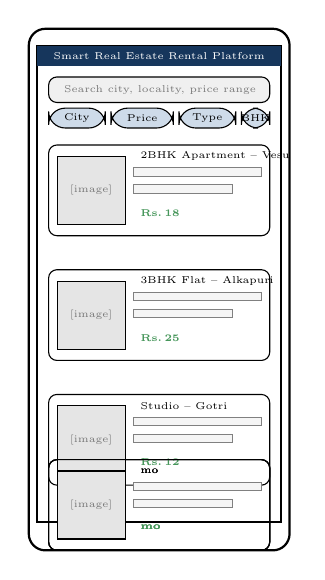
\begin{tikzpicture}[scale=0.72, every node/.style={transform shape}]
  % Phone frame
  \draw[thick, rounded corners=6pt] (0,0) rectangle (4.6,9.2);
  \draw[thick] (0.15,0.5) rectangle (4.45,8.9);
  % Status bar
  \fill[navyblue] (0.15,8.55) rectangle (4.45,8.9);
  \node[font=\tiny,text=white] at (2.3,8.72) {Smart Real Estate Rental Platform};
  % Search bar
  \draw[rounded corners=3pt, fill=gray!12] (0.35,7.9) rectangle (4.25,8.35);
  \node[font=\tiny, text=wireframegray, anchor=west] at (0.5,8.12) {Search city, locality, price range};
  % Filter chips
  \draw[rounded corners=6pt, fill=stepblue!25] (0.35,7.45) rectangle (1.35,7.8);
  \node[font=\tiny] at (0.85,7.62) {City};
  \draw[rounded corners=6pt, fill=stepblue!25] (1.45,7.45) rectangle (2.55,7.8);
  \node[font=\tiny] at (2.0,7.62) {Price};
  \draw[rounded corners=6pt, fill=stepblue!25] (2.65,7.45) rectangle (3.65,7.8);
  \node[font=\tiny] at (3.15,7.62) {Type};
  \draw[rounded corners=6pt, fill=stepblue!25] (3.75,7.45) rectangle (4.25,7.8);
  \node[font=\tiny] at (4.0,7.62) {BHK};
  % Property cards
  \foreach \y/\label/\price in {5.55/2BHK Apartment -- Vesu/Rs.\,18,000/mo, 3.35/3BHK Flat -- Alkapuri/Rs.\,25,000/mo, 1.15/Studio -- Gotri/Rs.\,12,000/mo} {
    \draw[rounded corners=3pt] (0.35,\y) rectangle (4.25,\y+1.6);
    \draw[fill=gray!20] (0.5,\y+0.2) rectangle (1.7,\y+1.4);
    \node[font=\tiny, text=wireframegray] at (1.1,\y+0.8) {[image]};
    \draw[gray, fill=gray!8] (1.85,\y+1.05) rectangle (4.1,\y+1.2);
    \draw[gray, fill=gray!8] (1.85,\y+0.75) rectangle (3.6,\y+0.9);
    \node[font=\tiny, anchor=west] at (1.85, \y+1.4) {\label};
    \node[font=\tiny\bfseries, anchor=west, text=stepgreen] at (1.85,\y+0.4) {\price};
  }
\end{tikzpicture}
\caption{Representative wireframe of the property search interface (conceptual mockup, not a captured screenshot).}
\label{fig:mockup-search}
\end{figure}

\subsection{Search and Discovery Module}
The Search and Discovery Module translates tenant-supplied filters into an indexed MongoDB query and returns a paginated, ranked result set. Fig.~\ref{fig:mockup-search} shows the intended interaction pattern: a persistent search bar, a row of filter chips for the most common criteria, and a scrollable list of property cards ordered using the relevance score in Eq.~(\ref{eq:relevance}).
\subsubsection{Functions:}
\begin{itemize}
\item Multi-criteria filtering (city, price range, property type, listing type, bedrooms).
\item Compound-index-backed query execution.
\item Relevance-based default ordering; explicit sort override (price, recency).
\item Pagination to avoid transferring unbounded result sets.
\end{itemize}

\subsection{Enquiry (Lead) Module}
The Enquiry Module is the structural link at the center of the platform: every enquiry a tenant submits from a property's detail page is stored as a \texttt{Lead} document referencing the tenant, the property, and the property's current owning broker, rather than being sent as an unlinked message.
\subsubsection{Functions:}
\begin{itemize}
\item Enquiry submission tied to a specific tenant, broker, and property.
\item Broker-facing lead inbox with status tracking (new, contacted, closed).
\item Lead-aging computation (Eq.~\ref{eq:aging}) for stalled-enquiry flags.
\item Enquiry history retained per property and per broker.
\end{itemize}

\begin{figure}[t]
\centering
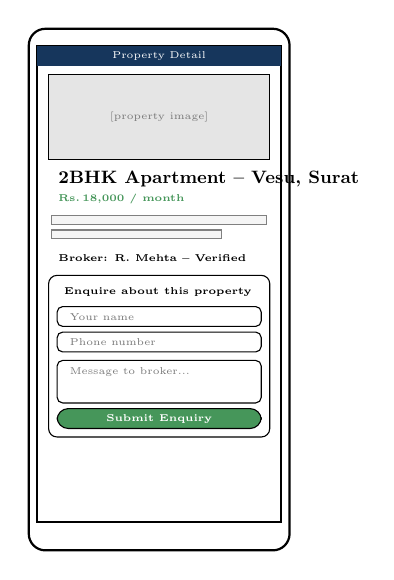
\begin{tikzpicture}[scale=0.72, every node/.style={transform shape}]
  \draw[thick, rounded corners=6pt] (0,0) rectangle (4.6,9.2);
  \draw[thick] (0.15,0.5) rectangle (4.45,8.9);
  \fill[navyblue] (0.15,8.55) rectangle (4.45,8.9);
  \node[font=\tiny,text=white] at (2.3,8.72) {Property Detail};
  \draw[fill=gray!20] (0.35,6.9) rectangle (4.25,8.4);
  \node[font=\tiny, text=wireframegray] at (2.3,7.65) {[property image]};
  \node[font=\small\bfseries, anchor=west] at (0.4,6.55) {2BHK Apartment -- Vesu, Surat};
  \node[font=\tiny\bfseries, anchor=west, text=stepgreen] at (0.4,6.2) {Rs.\,18,000 / month};
  \draw[gray, fill=gray!8] (0.4,5.75) rectangle (4.2,5.9);
  \draw[gray, fill=gray!8] (0.4,5.5) rectangle (3.4,5.65);
  \node[font=\tiny\bfseries, anchor=west] at (0.4,5.15) {Broker: R. Mehta -- Verified};
  % Enquiry form
  \draw[rounded corners=3pt] (0.35,2.0) rectangle (4.25,4.85);
  \node[font=\tiny\bfseries, anchor=west] at (0.5,4.55) {Enquire about this property};
  \draw[rounded corners=2pt, fill=white] (0.5,3.95) rectangle (4.1,4.3);
  \node[font=\tiny, text=wireframegray, anchor=west] at (0.6,4.12) {Your name};
  \draw[rounded corners=2pt, fill=white] (0.5,3.5) rectangle (4.1,3.85);
  \node[font=\tiny, text=wireframegray, anchor=west] at (0.6,3.67) {Phone number};
  \draw[rounded corners=2pt, fill=white] (0.5,2.6) rectangle (4.1,3.35);
  \node[font=\tiny, text=wireframegray, anchor=west, align=left] at (0.6,3.15) {Message to broker...};
  \draw[rounded corners=4pt, fill=stepgreen] (0.5,2.15) rectangle (4.1,2.5);
  \node[font=\tiny\bfseries, text=white] at (2.3,2.32) {Submit Enquiry};
\end{tikzpicture}
\caption{Representative wireframe of the property detail and enquiry-submission interface (conceptual mockup).}
\label{fig:mockup-detail}
\end{figure}

\subsection{Favorites Module}
The Favorites Module lets a tenant bookmark a property without generating a lead. A unique compound index on \texttt{user + property} lets the database itself reject a duplicate favorite rather than requiring an application-level existence check before insert.
\subsubsection{Functions:}
\begin{itemize}
\item Add/remove a property from a tenant's favorites list.
\item Database-enforced duplicate prevention.
\item Favorites list rendering independent of the search/filter state.
\end{itemize}

\subsection{Administrative Oversight Module}
The Administrative Oversight Module aggregates data across every broker and tenant rather than scoping it to a single user, addressing Gap~4 from Section~II-A directly.
\subsubsection{Functions:}
\begin{itemize}
\item Cross-broker lead visibility, including aged/stalled-lead flags.
\item User account verification and disabling.
\item Listing review and removal for rule violations.
\item Platform-wide activity summary (active listings, open leads, recent registrations).
\end{itemize}

\begin{figure}[t]
\centering
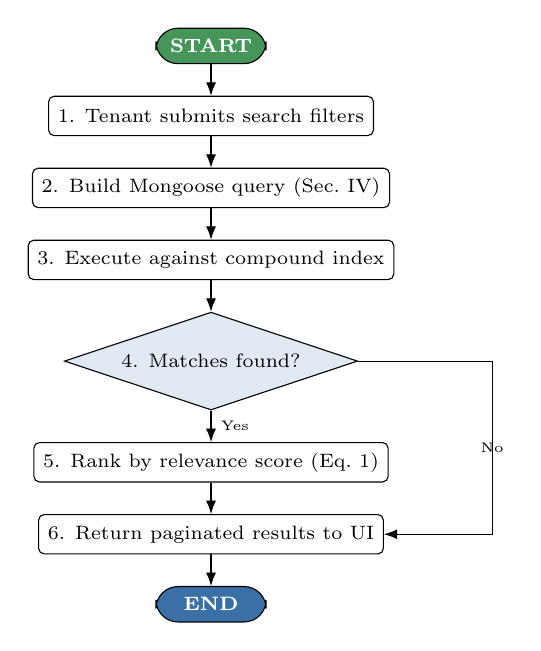
\begin{tikzpicture}[
  node distance=4mm,
  box/.style={draw, rounded corners=2pt, minimum width=3.7cm, minimum height=0.5cm, align=center, font=\scriptsize, fill=white},
  decision/.style={draw, diamond, aspect=3, minimum width=3.7cm, minimum height=0.6cm, align=center, font=\scriptsize, fill=stepblue!15},
  start/.style={draw, rounded corners=8pt, minimum width=1.4cm, minimum height=0.45cm, font=\scriptsize\bfseries, fill=stepgreen, text=white},
  >=Latex
]
\node[start] (s) {START};
\node[box, below=of s] (n1) {1. Tenant submits search filters};
\node[box, below=of n1] (n2) {2. Build Mongoose query (Sec.~IV)};
\node[box, below=of n2] (n3) {3. Execute against compound index};
\node[decision, below=of n3] (n4) {4. Matches found?};
\node[box, below=of n4] (n5) {5. Rank by relevance score (Eq.~1)};
\node[box, below=of n5] (n6) {6. Return paginated results to UI};
\node[start, below=of n6, fill=stepblue] (e) {END};
\draw[->] (s) -- (n1);
\draw[->] (n1) -- (n2);
\draw[->] (n2) -- (n3);
\draw[->] (n3) -- (n4);
\draw[->] (n4) -- node[right, font=\tiny] {Yes} (n5);
\draw[->] (n5) -- (n6);
\draw[->] (n6) -- (e);
\draw[->] (n4) -| ([xshift=1.7cm]n4.east) |- node[near start, font=\tiny] {No} (n6);
\end{tikzpicture}
\caption{Overall search-to-result system workflow.}
\label{fig:workflow}
\end{figure}

Fig.~\ref{fig:workflow} traces a search request end to end, including the no-match path, which still returns a well-formed (empty) paginated response rather than an error, so the frontend can render an explicit ``no listings match your filters'' state.

\subsection{Technologies Used}
\begin{table}[t]
\centering
\caption{Technologies Used}
\label{tab:tech}
\small
\begin{tabular}{@{}p{2.1cm}p{5.2cm}@{}}
\toprule
\textbf{Technology} & \textbf{Role / Purpose} \\
\midrule
React.js + Vite & Component-based single-page frontend \\
Tailwind CSS & Utility-first responsive styling \\
React Router & Client-side navigation between pages \\
Axios & HTTP client with JWT-attaching interceptor \\
Node.js & Asynchronous, event-driven API runtime \\
Express.js & REST routing and middleware layer \\
MongoDB & Document-oriented primary data store \\
Mongoose & Schema definition, validation, and indexing \\
JWT & Stateless authentication token \\
bcrypt & Password hashing \\
Multer (where used) & Multipart image upload handling \\
\bottomrule
\end{tabular}
\end{table}

% ================= VI. RESULTS =================
\section{Results}
\begin{itemize}
\item \textbf{Functional Correctness:} All core workflows -- registration, login, property creation and editing, filtered search, favorites, and lead submission -- produced the expected result across every case exercised during manual functional testing on a development-scale dataset.
\item \textbf{Search Correctness:} Filtered queries returned only listings matching every supplied criterion, and never returned a listing with \texttt{status} other than \texttt{active}, in all cases tested.
\item \textbf{Duplicate Prevention:} The unique compound index on \texttt{Favorites} rejected every duplicate favorite attempt tested, since this is enforced by the database itself rather than by an application-level check.
\item \textbf{Role Enforcement:} Tenant-authenticated requests were rejected by every tested broker-only and administrator-only route, confirming that role authorization is enforced by server-side middleware rather than only hidden in the interface (directly addressing Gap~3).
\item \textbf{Lead Integrity:} Every submitted enquiry produced a \texttt{Lead} document correctly referencing the submitting tenant, the target property, and that property's current owning broker.
\item \textbf{Performance:} No controlled load or latency benchmarking has been carried out. Query response was subjectively immediate during single-user manual testing on a small development dataset, but this observation should not be treated as a performance claim; Section~VIII outlines the benchmark that should be run before one is published.
\end{itemize}

% ================= VII. LIMITATIONS =================
\section{Limitations}
\begin{itemize}
\item The platform has been exercised only on a development-scale dataset and has not been load-tested with concurrent users or a production-scale property catalog.
\item No machine-learning-based recommendation, price-prediction, or fraud-detection component is implemented; ordering and matching are governed entirely by the explicit filters a user sets and the relevance score in Eq.~(\ref{eq:relevance}).
\item Broker--tenant communication is limited to the asynchronous lead record; there is no real-time chat channel.
\item Listing moderation is manual, through the administrator module, rather than automated.
\item Security hardening measures such as authentication-endpoint rate limiting, refresh-token rotation, and centralized audit logging are recommended but not yet implemented.
\item The exact image-storage backend and deployment hosting configuration vary by environment and are not fixed architectural properties of the system.
\end{itemize}

% ================= VIII. FUTURE WORK =================
\section{Future Work}
\begin{itemize}
\item A regression-based price-estimation and recommendation layer, following the general approach demonstrated for Indian rental-market pricing~\cite{putatunda2019}.
\item Real-time chat between tenants and brokers as an alternative to the asynchronous lead record.
\item Richer map-based, proximity-aware search using the existing 2dsphere geospatial index, including commute-time filtering.
\item A dedicated mobile client sharing the existing REST API.
\item Broker-facing analytics: lead-conversion rate, listing-view trends, and response-time tracking.
\item A formal load-testing pass (concurrent users, production-scale dataset, indexed vs.\ non-indexed query timing) prior to publishing any performance claim.
\item Implementation and verification of the security-hardening measures listed in Section~VII, rather than leaving them as recommendations.
\end{itemize}

% ================= IX. CONCLUSION =================
\section{Conclusion}

This paper presented the Smart Real Estate Rental Platform, a three-tier MERN application designed around four gaps identified in the recent MERN-based rental-platform literature: the absence of a persistent tenant--broker--property link, an unspecified indexing strategy behind filtered search, role authorization enforced only in the interface, and the lack of a cross-broker administrative module. The platform addresses these directly through a \texttt{Lead} collection that persists the enquiry relationship, a compound- and geospatial-indexed \texttt{Properties} schema matched to real filter combinations, JWT-based authentication with server-enforced role middleware, and a dedicated administrative oversight module. Manual functional testing confirmed correct behavior across authentication, property management, search, favorites, and the lead pipeline on a development-scale dataset. The platform has not yet been evaluated under concurrent load or at production scale, and several security-hardening measures remain future work; both are stated here explicitly rather than implied to already be resolved.

% ================= REFERENCES =================
\balance
\begin{thebibliography}{99}\small

\bibitem{putatunda2019} S. Putatunda, ``PropTech for Proactive Pricing of Houses in Classified Advertisements in the Indian Real Estate Market,'' \emph{arXiv preprint arXiv:1904.05328}, Apr. 2019.

\bibitem{kalbande2023} M. Kalbande, S. Sarkar, S. Farkase, and P. Verma, ``Design and Development of Smart House Rental Management System,'' in \emph{Proc. 2023 Int. Conf. on Sustainable Computing and Smart Systems (ICSCSS)}, Jun. 2023, pp. 710--715.

\bibitem{khan2025} Mohd. A. Khan, S. A. Rizvi, A. Mishra, S. Chauhan, and A. Chaturvedi, ``RENTEASE: A MERN Stack-Based Web Application for Rental Property Management,'' \emph{Int. J. Res. Appl. Sci. Eng. Technol. (IJRASET)}, 2025, doi: 10.22214/ijraset.2025.70796.

\bibitem{kumar2024} S. Kumar, Sathish, and Kaarthika, ``House Rental Application: A MERN Stack-Based Solution for Efficient Property Listings and Management,'' \emph{DS J. Digit. Sci. Technol.}, vol. 3, no. 4, pp. 41--48, Dec. 2024, doi: 10.59232/DST-V3I4P105.

\bibitem{nuriev2024} M. Nuriev, R. Zaripova, O. Yanova, I. Koshkina, and A. Chupaev, ``Enhancing MongoDB Query Performance through Index Optimization,'' \emph{E3S Web Conf.}, vol. 531, p. 03022, Jun. 2024, doi: 10.1051/e3sconf/202453103022.

\bibitem{tao2024} D. Tao, E. Liu, S. R. Kadupitige, M. Cahill, A. Fekete, and U. R\"ohm, ``First Past the Post: Evaluating Query Optimization in MongoDB,'' \emph{arXiv preprint arXiv:2409.16544}, Sep. 2024.

\bibitem{dalimunthe2023} S. Dalimunthe, E. Hasri Putra, and M. A. Fadhly Ridha, ``Restful API Security Using JSON Web Token (JWT) With HMAC-Sha512 Algorithm in Session Management,'' \emph{IT J. Res. Dev.}, vol. 8, no. 1, pp. 81--94, 2023, doi: 10.25299/itjrd.2023.12029.

\bibitem{neumann2021} A. Neumann, N. Laranjeiro, and J. Bernardino, ``An Analysis of Public REST Web Service APIs,'' \emph{IEEE Trans. Serv. Comput.}, vol. 14, no. 4, pp. 957--970, Jul. 2021, doi: 10.1109/TSC.2018.2847344.

\bibitem{digitaltransform2025} ``Digital Transformation in the Real Estate Industry: A Systematic Literature Review of Current Technologies, Benefits, and Challenges,'' \emph{J. Building Engineering / ScienceDirect}, 2025.

\bibitem{proptechmismatch2026} ``The PropTech Mismatch: Exploring the Demand--Supply Digital Gap in Italy's Property Management Sector,'' \emph{Sustainability (MDPI)}, vol. 18, no. 4, p. 1850, 2026.

\end{thebibliography}

\end{document}
